\documentclass{article}

% these packages let you do math
\usepackage{amsmath}
\usepackage{amssymb}

% we need these packages for fancy R tables
\usepackage{booktabs}
\usepackage{float}
\usepackage{colortbl}
\usepackage{xcolor}

% these packages play with the spacing/margins of the document. Uncomment the commands on lines 16 and 17 to see what they do.
\usepackage{a4wide}
\usepackage{setspace}
\usepackage{geometry}
\usepackage{parskip}
%\doublespacing
%\geometry{margin=1.5in}

% this package helps us with including images. Setting the graphics path makes it easier to refer to things in the \includegraphics command.
\usepackage{graphicx}
\graphicspath{ {../figures/} }

% make some hyperlinks using the \href command
\usepackage{hyperref}
\hypersetup{
    colorlinks=true,
    linkcolor=black,
    urlcolor=blue
}

% set the author, title, and date of the document. \maketitle adds it to the document.
\author{Patrick Massey}
\title{Hidden Curriculum Assignment}
\date{02/18/2022}

\begin{document}
\maketitle

\section*{Data}
I use a subset of data from the 1997 National Longitudinal Survey of Youth, which contains longitudinal data on individuals from 1997 to 2019. In particular I use observations from 2002 that focus on the incarceration status of an individual for that year. When analyzing the data I remove any individuals for which there is no incarceration information available, or if they began the year already incarcerated. After cleaning the data I am left with 8,621 observations. I then create an dummy indicator value for if the individual is incarcerated at all during the year. This indicator variable \textit{incarcerated} will be the variable of interest for the model.
\newpage
\section*{Empirical Analysis} 
In this analysis I seek to estimate the probability of an individual becoming incarcerated based on race and sex. Looking at Figure \ref{fig:graph} below, we see that Black Males have the highest incarceration rate of almost 6\%. Males in general have a higher incarceration rate than Females. One anomaly is for the Mixed Race (Non-Hispanic) group. This should be seen as an small sample size issue because out of the 8,621 observations Mixed Race (Non-Hispanic) make up 81 observations.
\begin{figure}[H]
    \begin{center}
        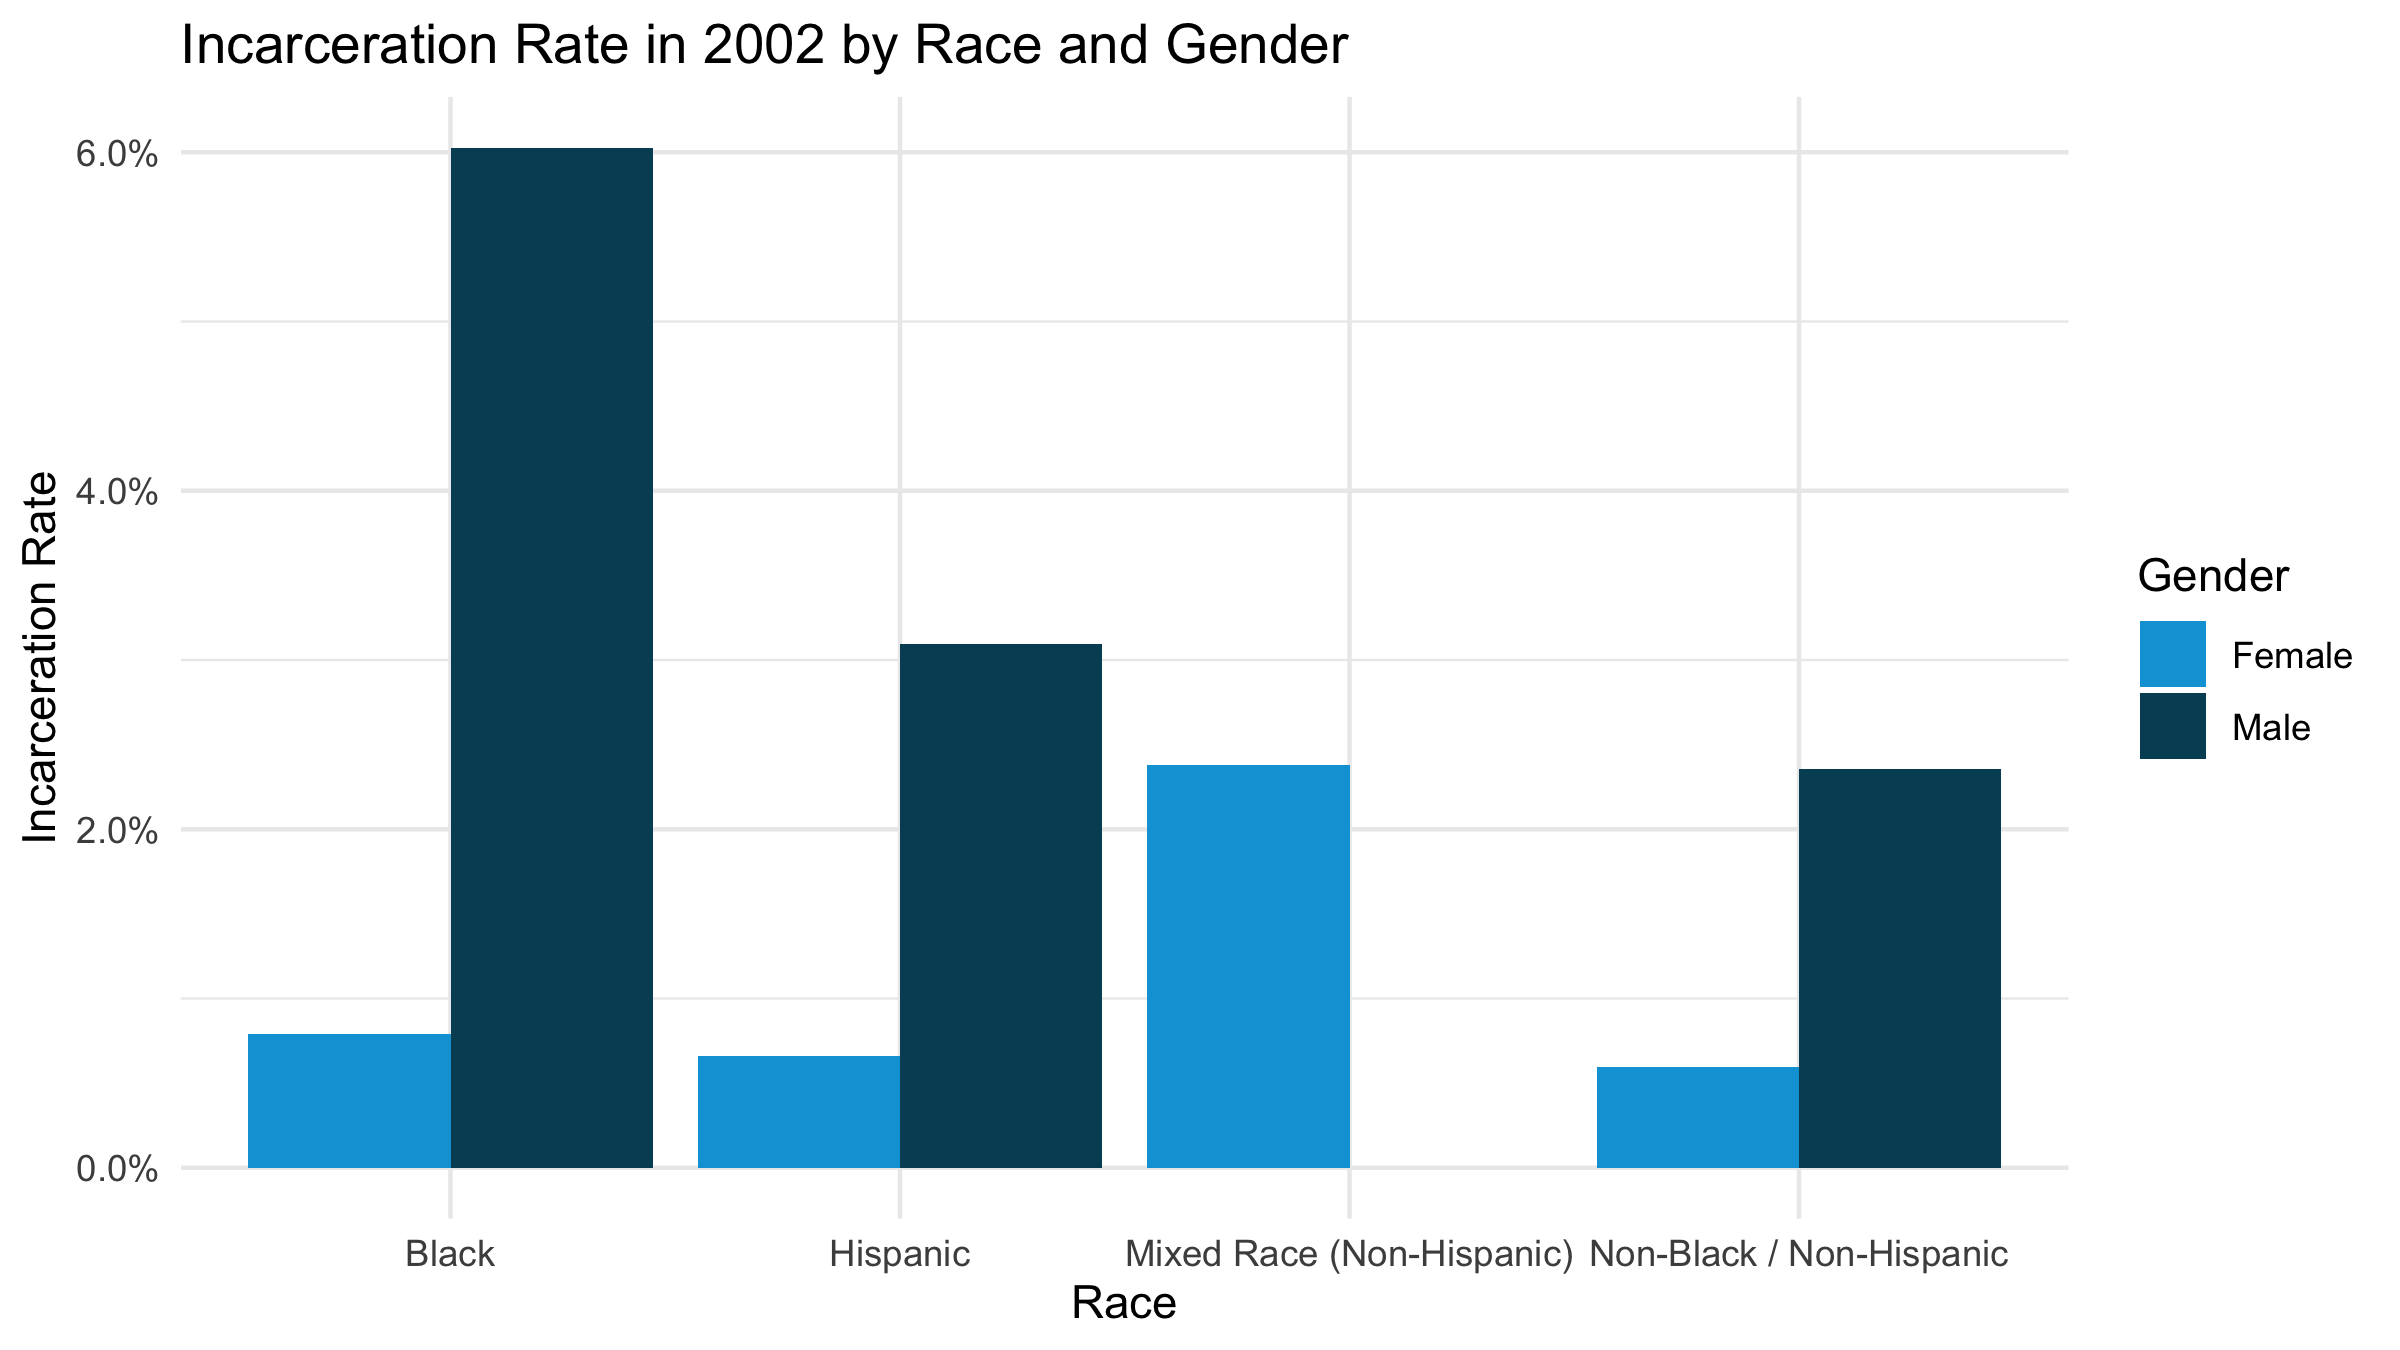
\includegraphics[width=.85\textwidth]{incarceration_rate_by_racegender}
    \end{center}
    \caption{Incarceration Rate in 2002 by Race and Gender}
    \label{fig:graph}
\end{figure}
I summarize the graph in Table \ref{tab:tab:summarystats} below which shows the incarceration rate broken down by sex and race.
\begin{table}[H]

\caption{\label{tab:tab:summarystats}Incarceration Rate in 2002 by Race and Gender}
\centering
\begin{tabular}[t]{lrrrr}
\toprule
Gender & Black & Hispanic & Mixed Race Non Hispanic & Non Black Non Hispanic\\
\midrule
\cellcolor{gray!6}{Female} & \cellcolor{gray!6}{0.0079225} & \cellcolor{gray!6}{0.0066225} & \cellcolor{gray!6}{0.0238095} & \cellcolor{gray!6}{0.0059798}\\
Male & 0.0602740 & 0.0309498 & 0.0000000 & 0.0235602\\
\bottomrule
\end{tabular}
\end{table}

\newpage
The model we are seeking to estimate is shown below:
\begin{equation*}
Y_i = \beta X_i 
\end{equation*}
Where $Y_i$ is a binary value for an individuals incarceration status and $X_i$ is a vector containing sex and race characteristics. I summarize the regression results in Table \ref{tab:regression} below.


% Table created by stargazer v.5.2.2 by Marek Hlavac, Harvard University. E-mail: hlavac at fas.harvard.edu
% Date and time: Mon, Feb 14, 2022 - 5:09:34 PM
\begin{table}[!htbp] \centering 
  \caption{Regression Output. Omitted category is Black Females.} 
  \label{tab:regression} 
\begin{tabular}{@{\extracolsep{5pt}}lc} 
\\[-1.8ex]\hline 
\hline \\[-1.8ex] 
 & \multicolumn{1}{c}{\textit{Dependent variable:}} \\ 
\cline{2-2} 
\\[-1.8ex] & Incarcerations in 2002 \\ 
\hline \\[-1.8ex] 
 Hispanic & $-$0.015$^{***}$ \\ 
  & (0.005) \\ 
  & \\ 
 Mixed Race (Non-Hispanic) & $-$0.021 \\ 
  & (0.013) \\ 
  & \\ 
 Non-Black / Non-Hispanic & $-$0.019$^{***}$ \\ 
  & (0.004) \\ 
  & \\ 
 Male & 0.028$^{***}$ \\ 
  & (0.003) \\ 
  & \\ 
 Constant & 0.020$^{***}$ \\ 
  & (0.003) \\ 
  & \\ 
\hline \\[-1.8ex] 
Observations & 8,621 \\ 
R$^{2}$ & 0.012 \\ 
Adjusted R$^{2}$ & 0.012 \\ 
Residual Std. Error & 0.141 (df = 8616) \\ 
F Statistic & 27.193$^{***}$ (df = 4; 8616) \\ 
\hline 
\hline \\[-1.8ex] 
\textit{Note:}  & \multicolumn{1}{r}{$^{*}$p$<$0.1; $^{**}$p$<$0.05; $^{***}$p$<$0.01} \\ 
\end{tabular} 
\end{table} 


All variables are statistically significant at the 99\% level except for Mixed Race (Non-Hispanic) category which I believe goes back to the small $n$ issue.

Analyzing the regression results we can see that there appears to be racial discrimination towards Black individuals as every other racial group shows a constant that is less than or equal to 0. This indicates that simply being Black shows higher risk of incarceration. We also see that Black Males show higher risk for incarceration than Black Females which matches the trends in the data.
\end{document}
